\documentclass[11pt]{article}
\usepackage[T1]{fontenc}
\usepackage{fullpage,graphicx,psfrag,amsmath,amsfonts}
\usepackage[small,bf]{caption}
\usepackage[utf8]{inputenc}
\usepackage[english]{babel}
\usepackage{lipsum}
\usepackage{url}
\usepackage{bm}
\usepackage{float}
\usepackage{physics}
\usepackage{lmodern}
\usepackage{enumitem}
\usepackage{indentfirst}
\usepackage{setspace} 
\usepackage[left=25mm, right=25mm]{geometry}
\newtheorem{theorem}{Theorem}
\onehalfspacing

\begin{document}
\begin{center} 
    \textbf{\LARGE Minimal Autocalibration Pipeline}

    \vspace{0.5cm}
    A minimal approach and experiments
            
    \vspace{1.5cm}

    \textbf{Filippo Grotto VR460638 \\ Matteo Meneghetti VR469054}

    \vspace{0.5cm}
    Master degree in Computer Engineering for Robotics and Smart Industry

    \vfill
            
    Computer Vision 2021/2022
            
    \vspace{0.8cm}
                
    Department of Computer Science\\
    University of Verona\\
            
\end{center}

\tableofcontents

\newpage
\section{Problem Statement}
The main idea of this project is to present a minimal pipeline to estimate intrinsic camera parameters using auto-calibration methods. We will assume known corresponding points and an initial estimation of the intrinsic camera parameters. The entire pipeline is based on a dataset provided by Zephyr, in particular, we used 3DFlow Dante dataset \cite{Dante}.

\section{Pipeline}
The pipeline is composed of two separate steps the first one to load the dataset and prepare a dedicated data-structure and the last one to perform the actual auto-calibration steps that will be discussed. The related files are \textit{pipeline\_dataset.m} and \textit{pipeline\_autocal.m}, respectively. Assuming the dataset provided by Zephyr with \textit{Visibility.txt}. The only requirements for running those scripts are the \textit{directory} variables defined on top of both.

\subsection{Data Structure}
Prepare the data structure from the Zephyr dataset. The idea is to build a node for each pair of images i, j with the related 3D point and the projected $(uv,vv)$ in the images i and j called correspondence points. Moreover the related rotations $R$, translations $t$ and the original intrinsic parameters $K$ are collected starting from the \textit{.xmp} files. In this way a symmetric cell $S\{i,j\}$ can be constructed. An example and instance for $S\{i,j\}$ is reported:
\begin{verbatim}
           points: [2147×3 double]
           uv_i: [2147×1 double]
           vv_i: [2147×1 double]
           uv_j: [2147×1 double]
           vv_j: [2147×1 double]
           name_view_i: '_SAM1001.JPG'
           name_view_j: '_SAM1002.JPG'
           K_i: [3×3 double]
           R_i: [3×3 double]
           t_i: [3×1 double]
           K_j: [3×3 double]
           R_j: [3×3 double]
           t_j: [3×1 double]
\end{verbatim}
Where \textit{points} are the 3D points, \textit{uu\_i} and \textit{vv\_i} define a point on the image pixels i, \textit{uv\_j} and \textit{vv\_j} define a point on the image pixels j, \textit{name\_view\_i} and \textit{name\_view\_j} are the filenames of the related images and finally the parameters of the cameras for i and j.

\subsection{Use centroids to select 3D points}
Using the corresponding points of a pair of images it is possible to estimate the fundamental matrices. In order to make this estimation robust, only the 3D points close enough to the centroid are considered. The basic idea is the following:
\begin{equation}
    || p - m || < \epsilon
\end{equation}
where $p$ is the point, $m$ is the mean of all points and $\epsilon = 3$ is the distance. Only the points close enough to the mean are selected. This selection is performed in the construction of the data-structure to reduce the number of edge cases in the computation.

\subsection{Fundamental Matrices}
The fundamental matrix is defined as:
\begin{equation}
    m'^TFm = 0.
\end{equation}
meaning that the corresponding point of $m$ in the the second image should be in the epipolar line described by $Fm$. We can also observe that $det(F) = 0$ since $det([e']_x) = 0$ and that the definition of $F$ is true even if we multiply by a scaling factor. The fundamental matrix is the relation of the pixel coordinates of the conjugate points. We can briefly mention this relation:
\begin{equation}
    F = K'^{-T}EK^{-1}
\end{equation}
The computation of the fundamental matrices can be performed using the pixel coordinates instead of normalized coordinates in the 8 points algorithm. The only property is the fact that $F$ should be singular. 

\bigskip
The problem of the 8 points linear algorithm is the sensitivity to noise and instability (ill-conditioned). Hartley proposed to use a standardization to improve the results \cite{Hartley95}. This can be performed by translating the points so that their origin matches and then scale them to get a mean distance of $\sqrt2$.
Given $T$ and $T'$ the transformations of $\bar{m} = Tm$ and $\bar{m}' = T'm'$. If we use the points $\bar{m}$ and $\bar{m}'$ in the eight points algorithm we can compute $\bar{F}$ and recover the original fundamental matrix with $F = T'^{T}\bar{F}T$. Finally, the estimation of the linear algorithm can be refined using a geometric residual equal to the sum of the distances between points and conjugate epipolar lines.
\begin{equation}
    min_{F} 
 \sum_{j} d(Fm_i, m_i')^2 + d(F^Tm_i'm_i)^2
\end{equation}
where $d()$ is the distance point-line in the cartesian plane \cite{Luong}.
\subsection{Epipolar lines}
\begin{figure}[H]
    \centering
    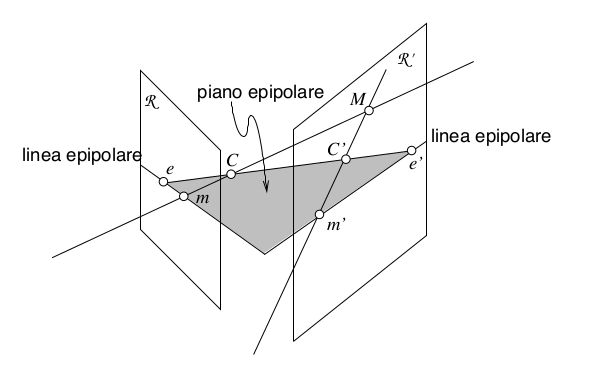
\includegraphics[scale=0.4]{images/epipolar.png}
    \caption{Epipolar geometry taken from \cite{Fusiello}}
    \label{fig:epipolar_geom}
\end{figure}
The main ideas are collected in the Longuet-Higgins equation which is reported considering two projection perspective matrices $P = [Q|q]$ and $P' = [Q'|q']$:
\begin{equation}
    0 = m'^T[e']_xQ'Q^{-1}m
\end{equation}
which can be rewritten with the relation of the fundamental matrix:
\begin{equation}
    m'^TFm = 0
\end{equation}
in fact if we consider $m$, the epipolar line is $Fm$. In Fig \ref{fig:epipolar} and \ref{fig:epipolar2} some examples obtained drawing the epipolar lines in both directions are reported to validate the experimental results.
\begin{figure}[H]
    \centering
    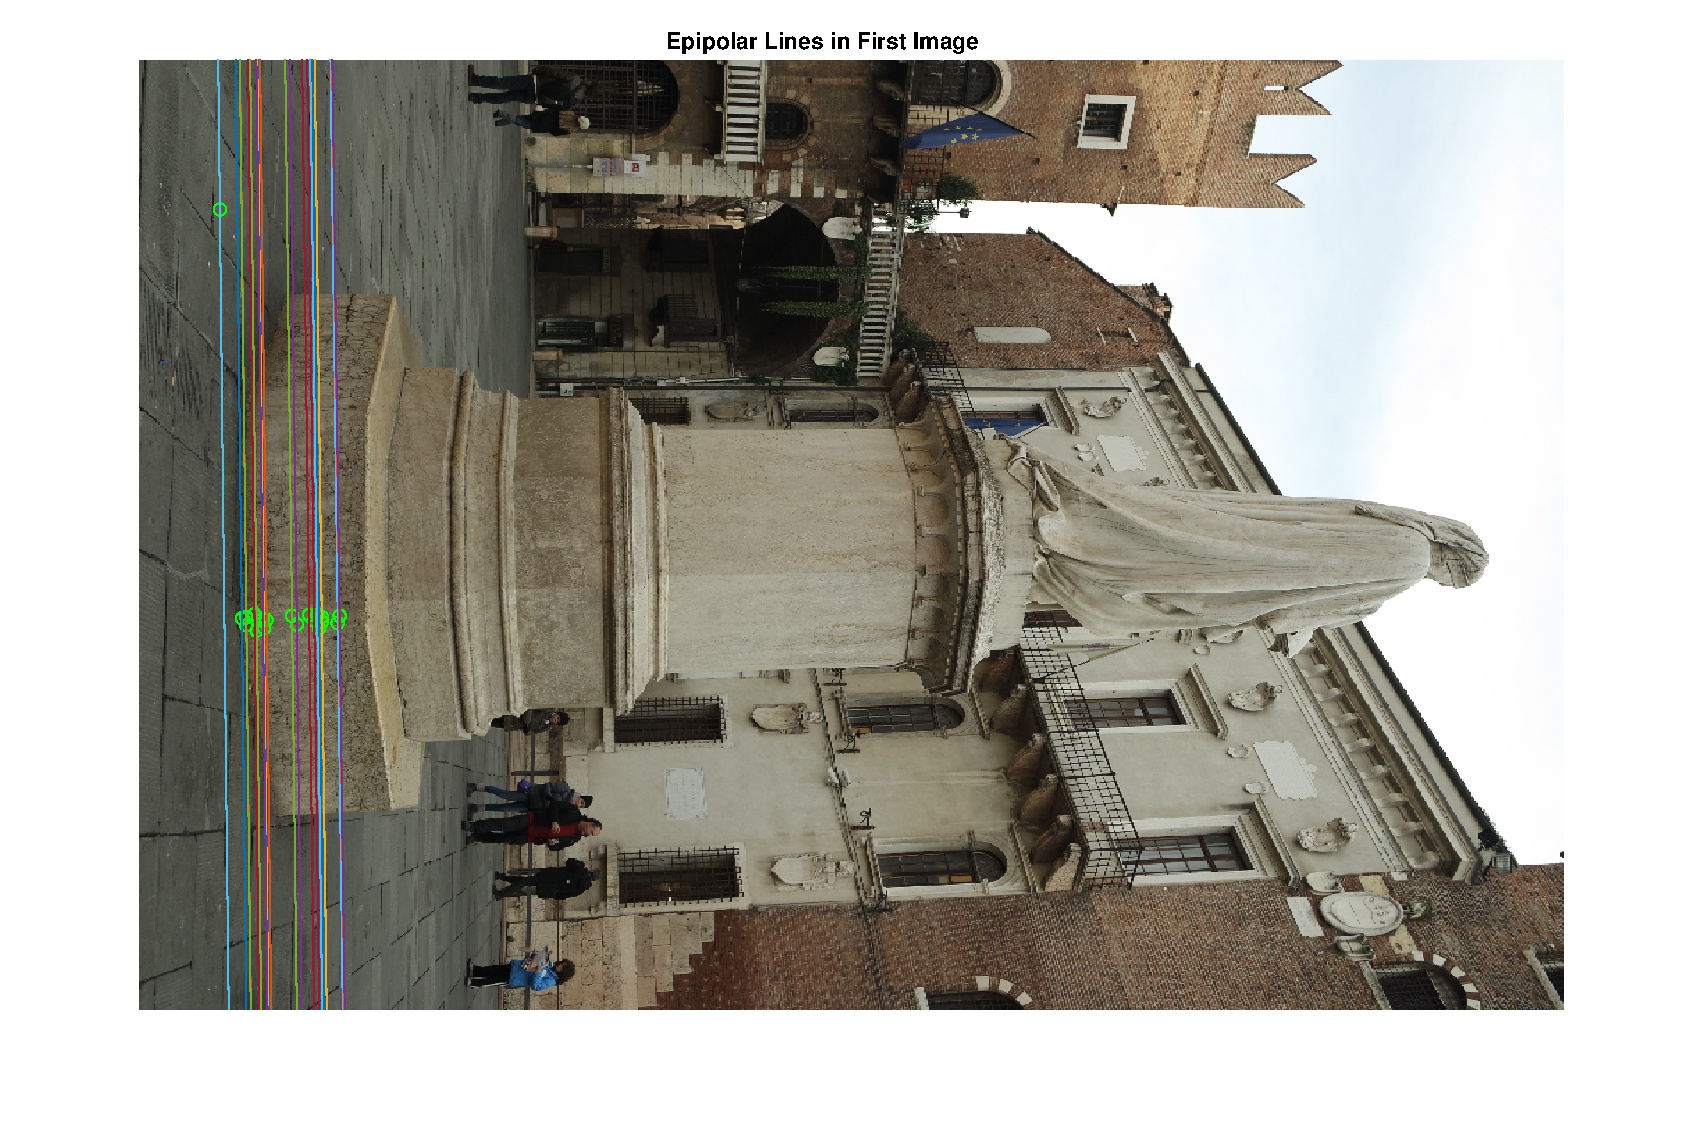
\includegraphics[scale=0.5]{images/epipolar1.eps}
    \qquad
    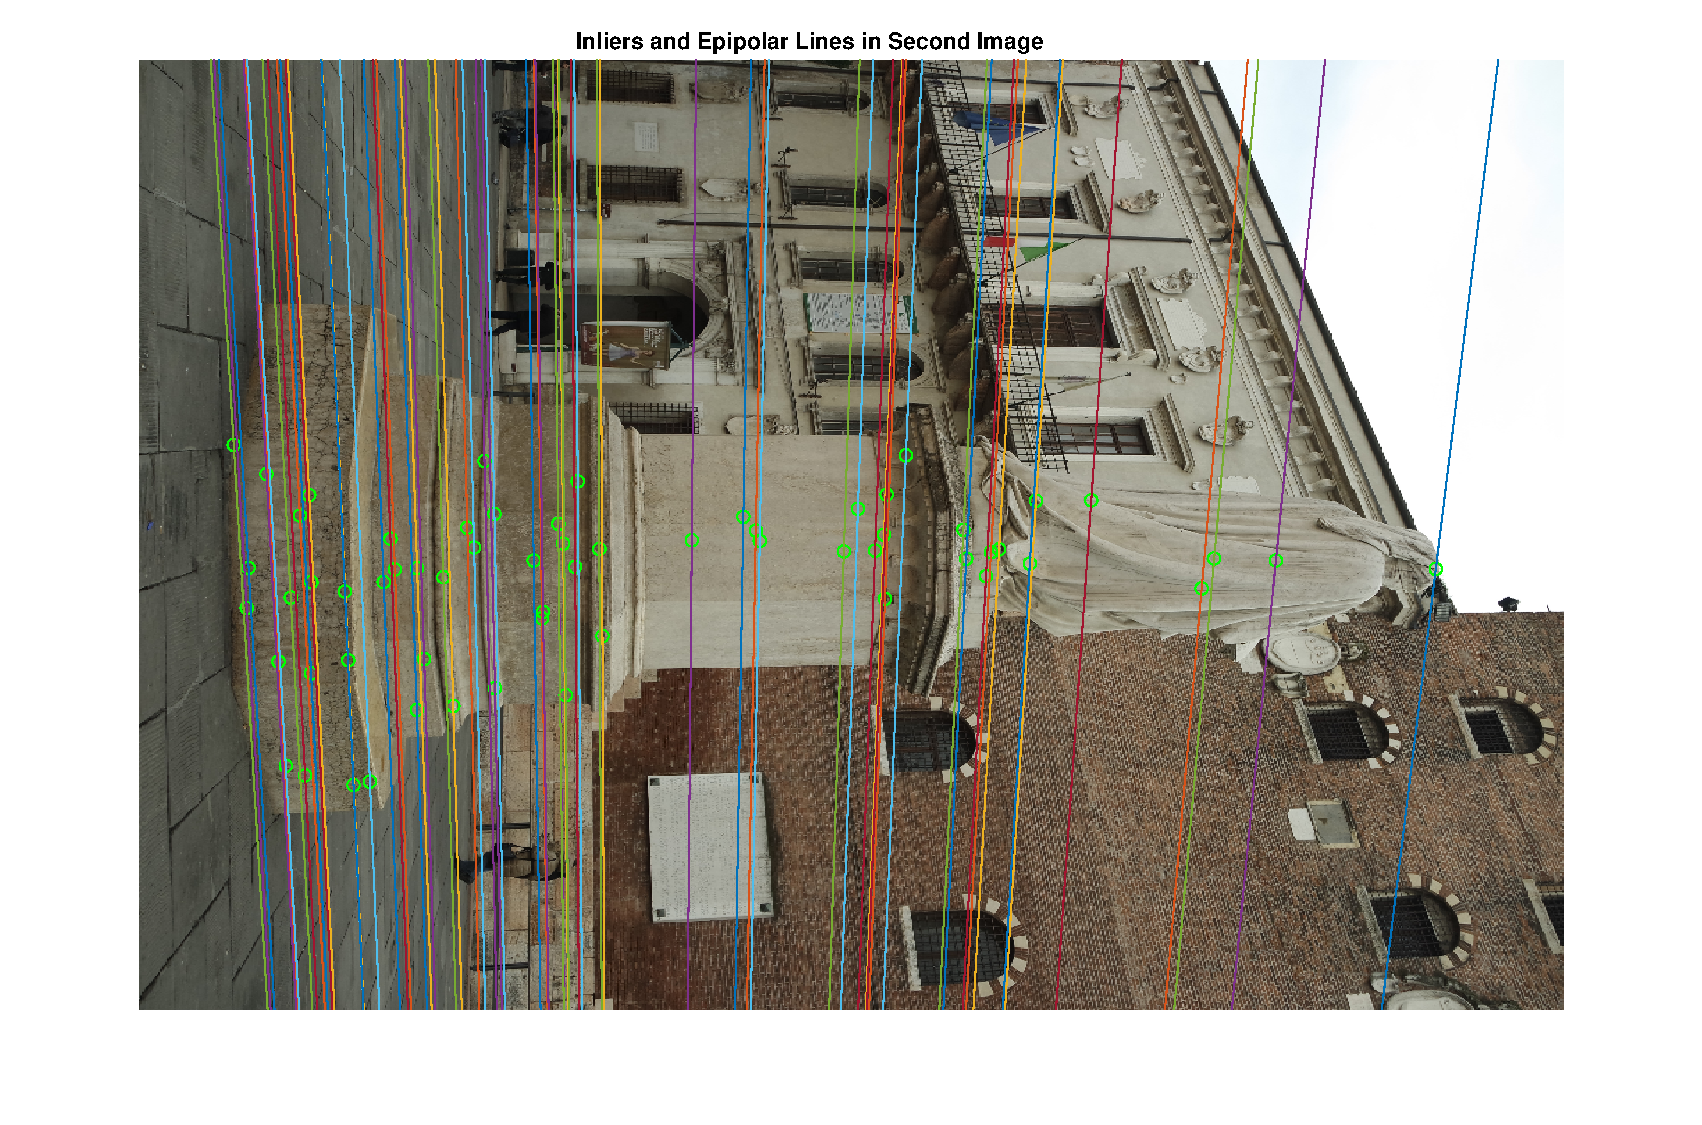
\includegraphics[scale=0.5]{images/epipolar2.eps}
    \caption{Epipolar lines of pair of images 1 and 2. It is visible the effect of the selection of 3D points}
    \label{fig:epipolar}
\end{figure}

\begin{figure}[H]
    \centering
    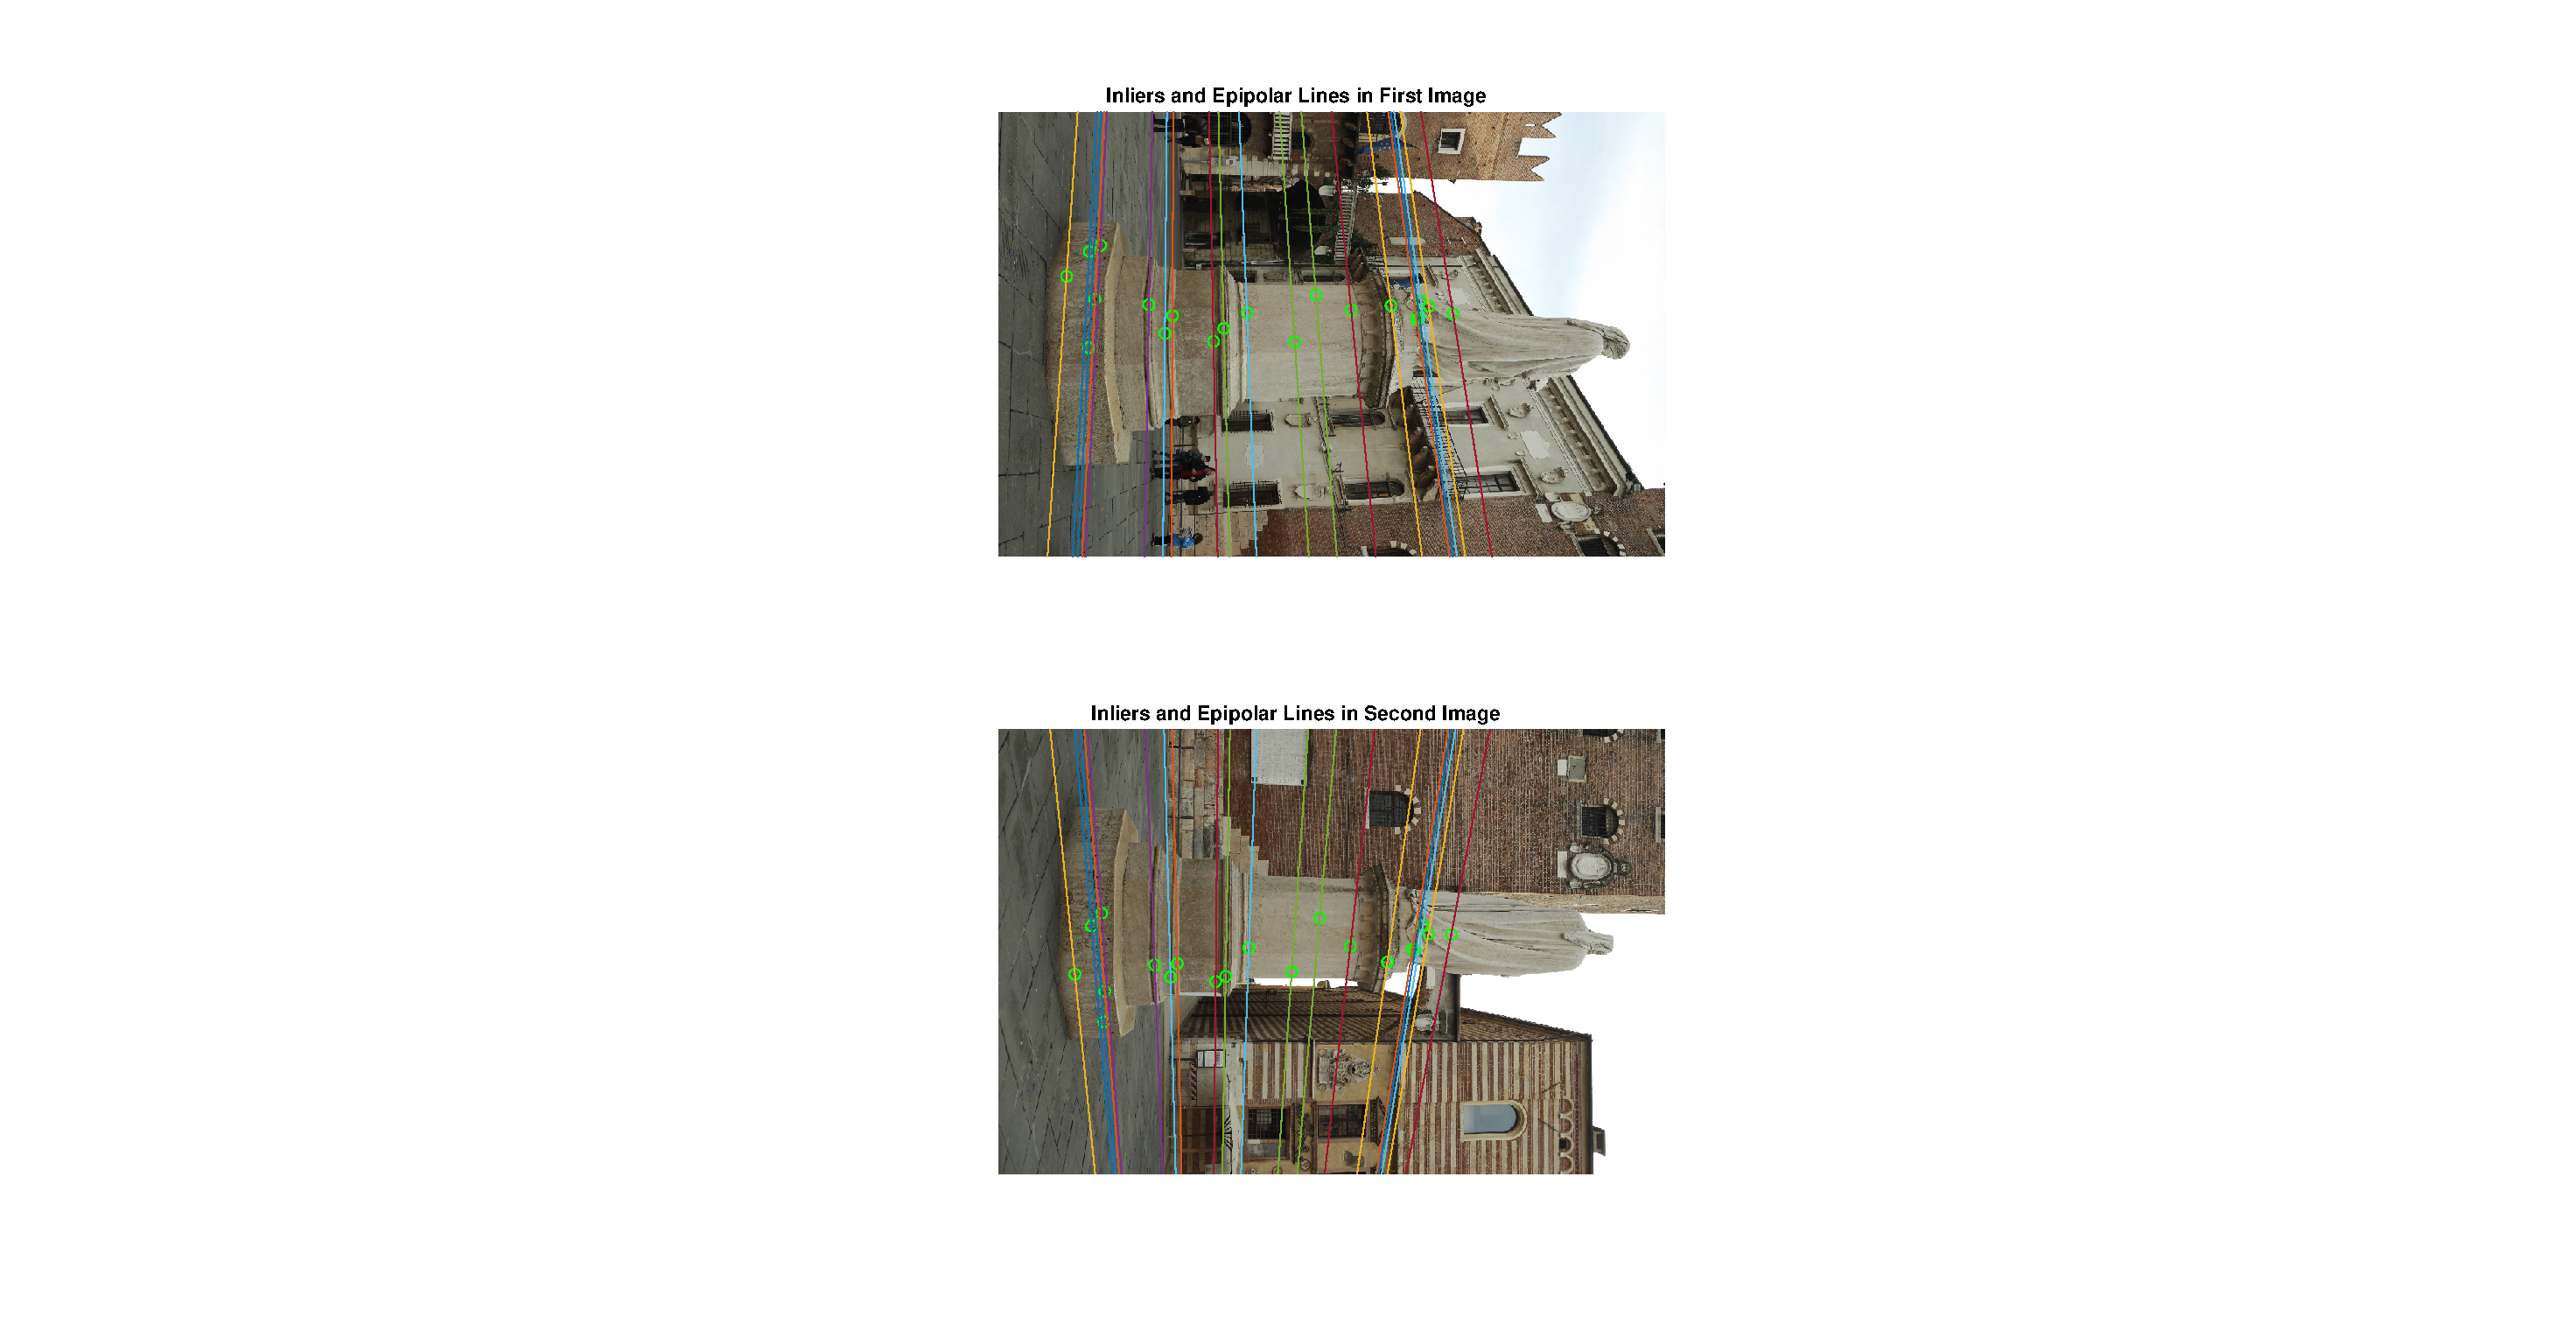
\includegraphics[scale=0.5]{images/epipolar3.eps}
    \qquad
    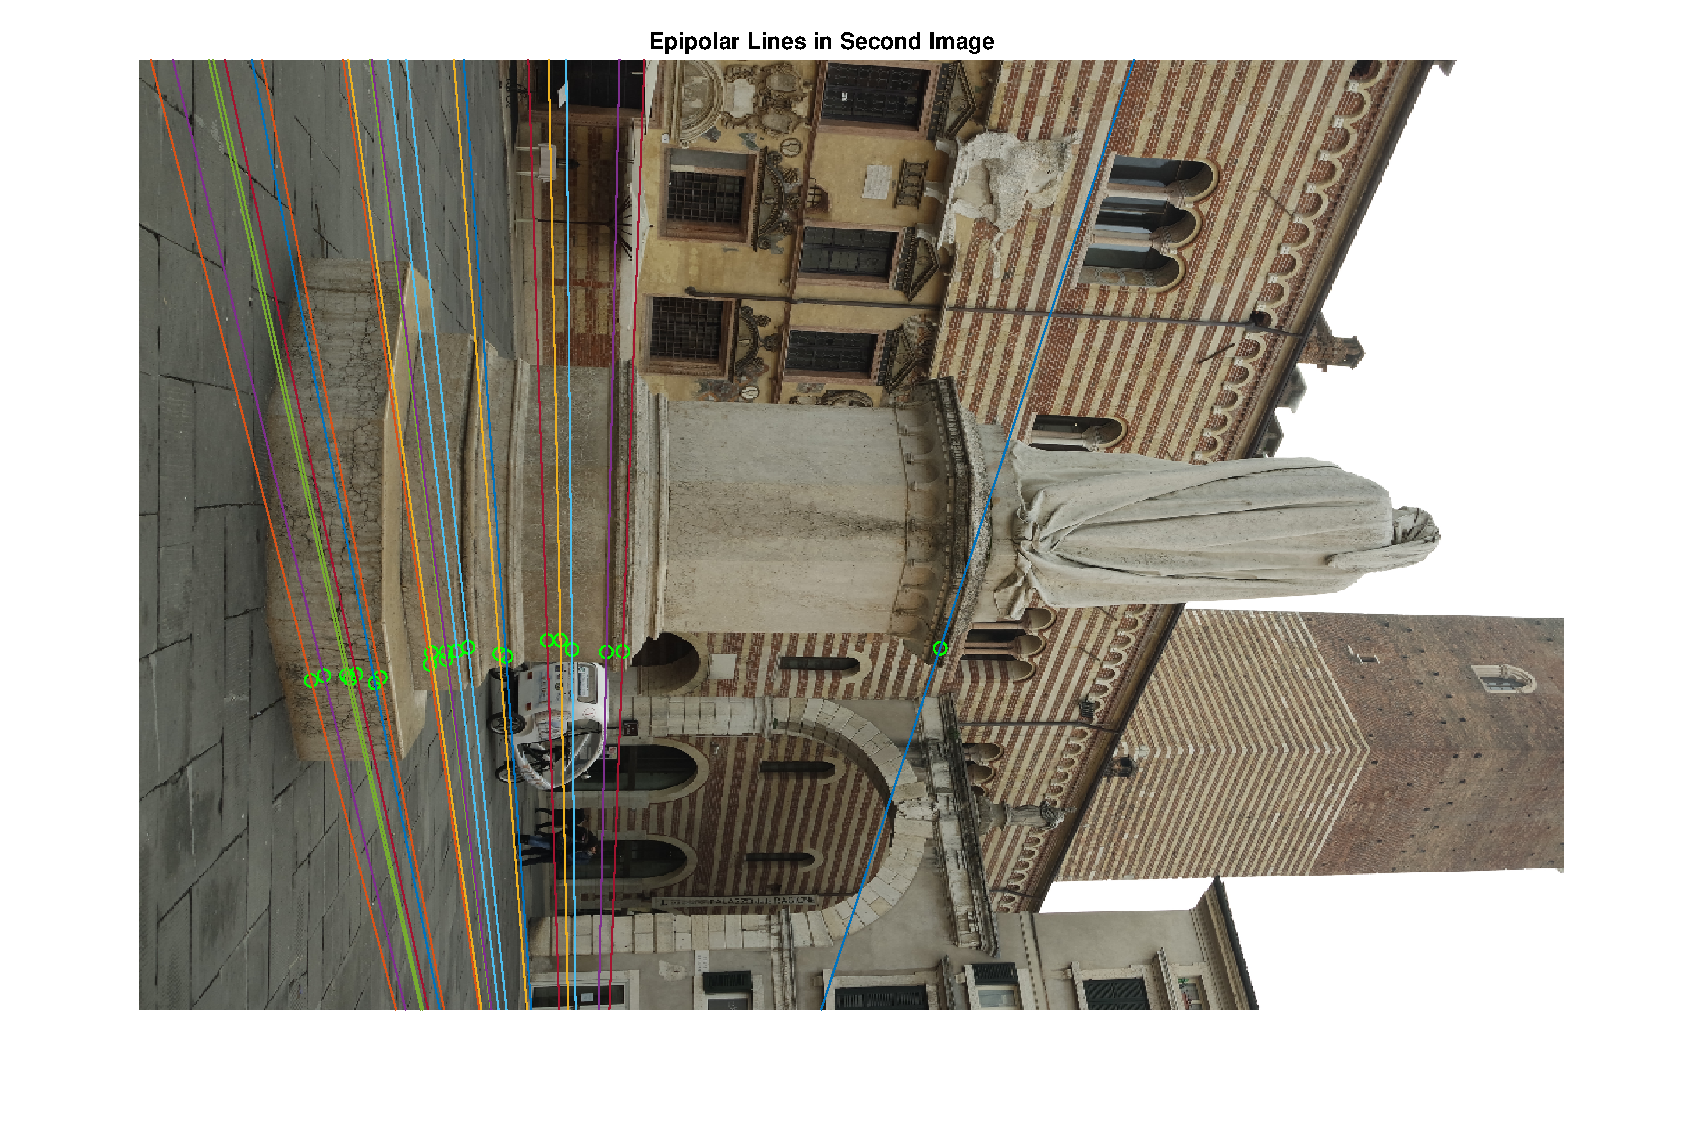
\includegraphics[scale=0.5]{images/epipolar4.eps}
    \caption{Epipolar lines of pair of images. It is visible the effect of the selection of 3D points}
    \label{fig:epipolar2}
\end{figure}


\subsection{Autocalibration}
Given the fundamental matrices the auto-calibration algorithms require an initial estimation of the matrix $K_0$ of internal camera parameters. A simple script is provided in \textit{compute\_k0.m} which extract the intrinsic camera parameters from the size of the image and the header information assuming a $35$mm focal length. An example of initial estimation is reported:
\begin{equation*}
K_0 = 1000 \begin{bmatrix}
    5.9410   &      0   & 2.7360\\
         0   & 5.9410    &1.8240\\
         0    &     0    &0.0010\\
    
        \end{bmatrix}
\end{equation*}
which is very close to the original values computed in Zephyr:
\begin{equation*}
    K = 1000 \begin{bmatrix}
     5.7942 &        0 &   2.7923\\
          0  &  5.7942  &  1.8174\\
          0  &       0  &  0.0010\\
        \end{bmatrix}
    \end{equation*}
\subsubsection{Medonca-Cipolla autocalibration}
A first simple calibration method was proposed by Medonca and Cipolla in \cite{Medonca99}. Considering the intrinsic parameters parametrized as
\begin{equation}
    K = \begin{bmatrix}
        \alpha_x & s & u_0 \\
        0   & \epsilon\alpha_x & v_0 \\
        0 & 0 & 1
    \end{bmatrix}
\end{equation}
where $\alpha_x$ is the product of the focal length and the magnification factor, $\begin{bmatrix}
    u_0 & v_0
\end{bmatrix}^T$ are the coordinates of the principal point, $s$ is the skew and $\epsilon$ is the aspect ratio. The main idea is to consider the following cost function for $n$ images:
\begin{equation}
    C(K_i, i = 1,\dots, n) = \sum_{ij}^{n} \frac{w_{ij} (\sigma_{1ij}-\sigma_{2ij})}{\sum_{kl}^{n}w_{kl} \sigma_{2ij}}
\end{equation}
where $\sigma_{1ij}$ and $\sigma_{2ij}$ are the non zero singular values of $K_j^TF_{ij}K_j$ in descending order, considering the fundamental matrix between two images i, j as $F_{ij}$ and the intrinsic parameters $K_j$. The weights $w_{ij}$ are the degree of confidence in the estimation of the fundamental matrix and can be equal to the number of points used in the computation of the fundamental matrix.

\bigskip
The implementation of this method is provided in \textit{cost\_medonca\_cipolla.m} and can be used with $lsqnonlin$ or $fmincon$ to solve the related minimization problem. Several parameters has been tested but using the computed fundamental matrices and initial estimation the solver produces the following intrinsic parameters matrix with an error of $2.1854\%$:
\begin{equation}
    K = 1000 \begin{bmatrix}
 
     5.9209  &  0.0017    &2.7613\\
          0  &  5.8837   & 1.8216\\
          0  &       0  &  0.0010\\ 
\end{bmatrix}
\end{equation}
\subsubsection{Kruppa method autocalibration}
The second calibration method proposed is Kruppa method that can be found in \cite{Prapitasari14} \cite{Pollefeys}. From the classical Kruppa's equations and cost function can be derived to be solved as a nonlinear least-squares optimization problem:
\begin{equation}
    C(K_i, i = 1,\dots, n) = \sum_{ij}^{n} \norm{\frac{F_{ij}w^{-1}F_{ij}^T}{||F_{ij}w^{-1}F_{ij}^T||} - \frac{[e_{ji}]_xw^{-1}[e_{ji}]^T}{||[e_{ji}]_xw^{-1}[e_{ji}]^T||}}
\end{equation}
where $F_{ij}$ are the fundamental matrices, $e$ are the epipoles and $w^{-1} = KK^T$. The norms used are the frobenius norms.

\bigskip
The implementation of this method is provided in \textit{cost\_kruppas\_method.m} and can be used with $lsqnonlin$ or $fmincon$ to solve the related minimization problem. Several parameters has been tested but using the computed fundamental matrices and initial estimation the solver produces the following intrinsic parameters matrix with an error of $2.5332\%$:
    \begin{equation}
        K = 1000 \begin{bmatrix}
     
     5.9410  &  0.0022   & 2.7361\\
          0  &  5.9409   & 1.8256\\
          0  &       0   & 0.0010\\
\end{bmatrix}
\end{equation}
\newpage
\subsubsection{Medonca-Cipolla toolbox}
The last calibration method is provided in the Computer Vision Toolbox from Andrea Fusiello. The main idea is the following theorem from Huang and Faugeras \cite{Faugeras89}
\begin{equation}
    det(E) = 0 \qquad \text{and} \qquad tr((EE^T))^2 - 2 tr((EE^T)^2) = 0
\end{equation}
The previous equation is a condition to have one singular value equal to zero for $E$ and two identical non-zero singular values. This condition can be used to build a cost function like:
\begin{equation}
    C(K_i, i = 1,\dots, n) = \sum_{i=1}^{n} \sum_{j=i+1}^{n} w_{ij} (tr((EE^T))^2 - 2 tr((EE^T)^2))^2
\end{equation}
where $E_{ij} = K'F_{ij}K$ and $w_ij$ are the degree of confidence in the estimation of the fundamental matrix. The cost function is minimized with the matlab algorithms like the previous algorithms but the convergence is not guaranteed for each initial value. An example obtained with this procedure is reported with an error of $0.64652\%$:
\begin{equation}
    K = 1000 \begin{bmatrix}
     5.8317  &       0   & 2.7673\\
          0  &  5.8317   & 1.8225\\
          0  &       0   & 0.0010\\ 
\end{bmatrix}
\end{equation}

\bigskip
\subsubsection{Autocalibration considerations}
As it is visible the auto-calibration algorithms improve the initial estimation based on the fundamental matrices provided. It is important to notice that both the initial estimation and the fundamental matrices play a big role on this estimation and its convergence. Another important considerations is related to the fact that the selecting points close to the mean is mandatory to have a robust estimation. Finally, the non-linear least square solver requires fine tuning to improve the accuracy of auto-calibration algorithms, in particular tolerances.

\newpage
\section{Relative orientation and 3D points evaluation}
Finally the relative orientation for each pair of images $(i,j)$ is recovered using the estimated $K$ with the function provided in the computer vision toolbox. The rotation $R_{ji}$ and translation $t_{ji}$ are saved in the related instance $S{i,j}$. Finally the absolute orientation is recovered using the original 3D points and the triangulated 3D points from corresponding points. The orthogonal procrustes problem (opa) is solved to recover the scaling, the rotation and the translation as follow:
\begin{equation}
    D=s(RM+t)
\end{equation}
the actual algorithm is not reported and can be found in th CV toolbox. Another possibility is to concatenate the relative orientation of each view with respect to the first one, triangulate the points and register them with iterative closest point algorithm (icp). However, the latter approach is not as robust as solving opa, it is computationally more expensive and it is not always possible to concatenate close views due to missing common points to compute the fundamental matrices.

\bigskip
In Fig \ref{fig:relative} the results of relative orientations and opa are reported to check the results obtained. In Fig \ref{fig:statue} the final result is reported using the inliers points of 5 views and the estimated $K$.
\begin{figure}[H]
    \centering
    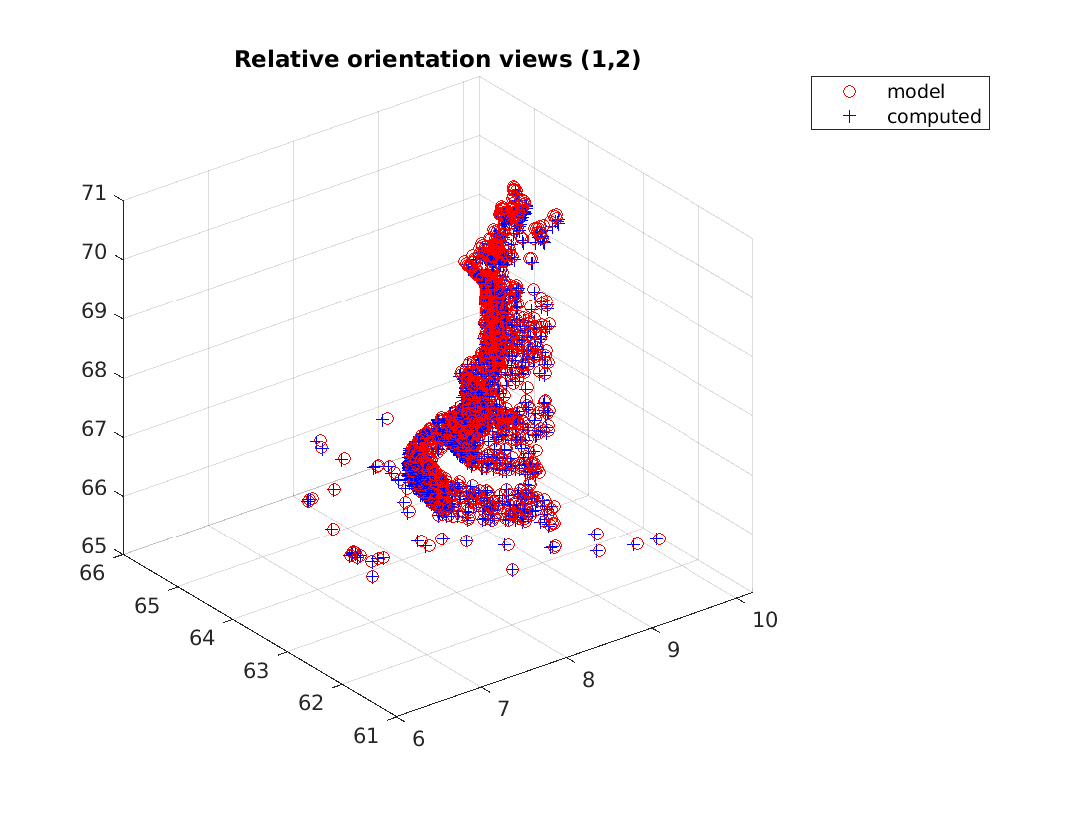
\includegraphics[scale=0.45]{images/relative_1.eps}
    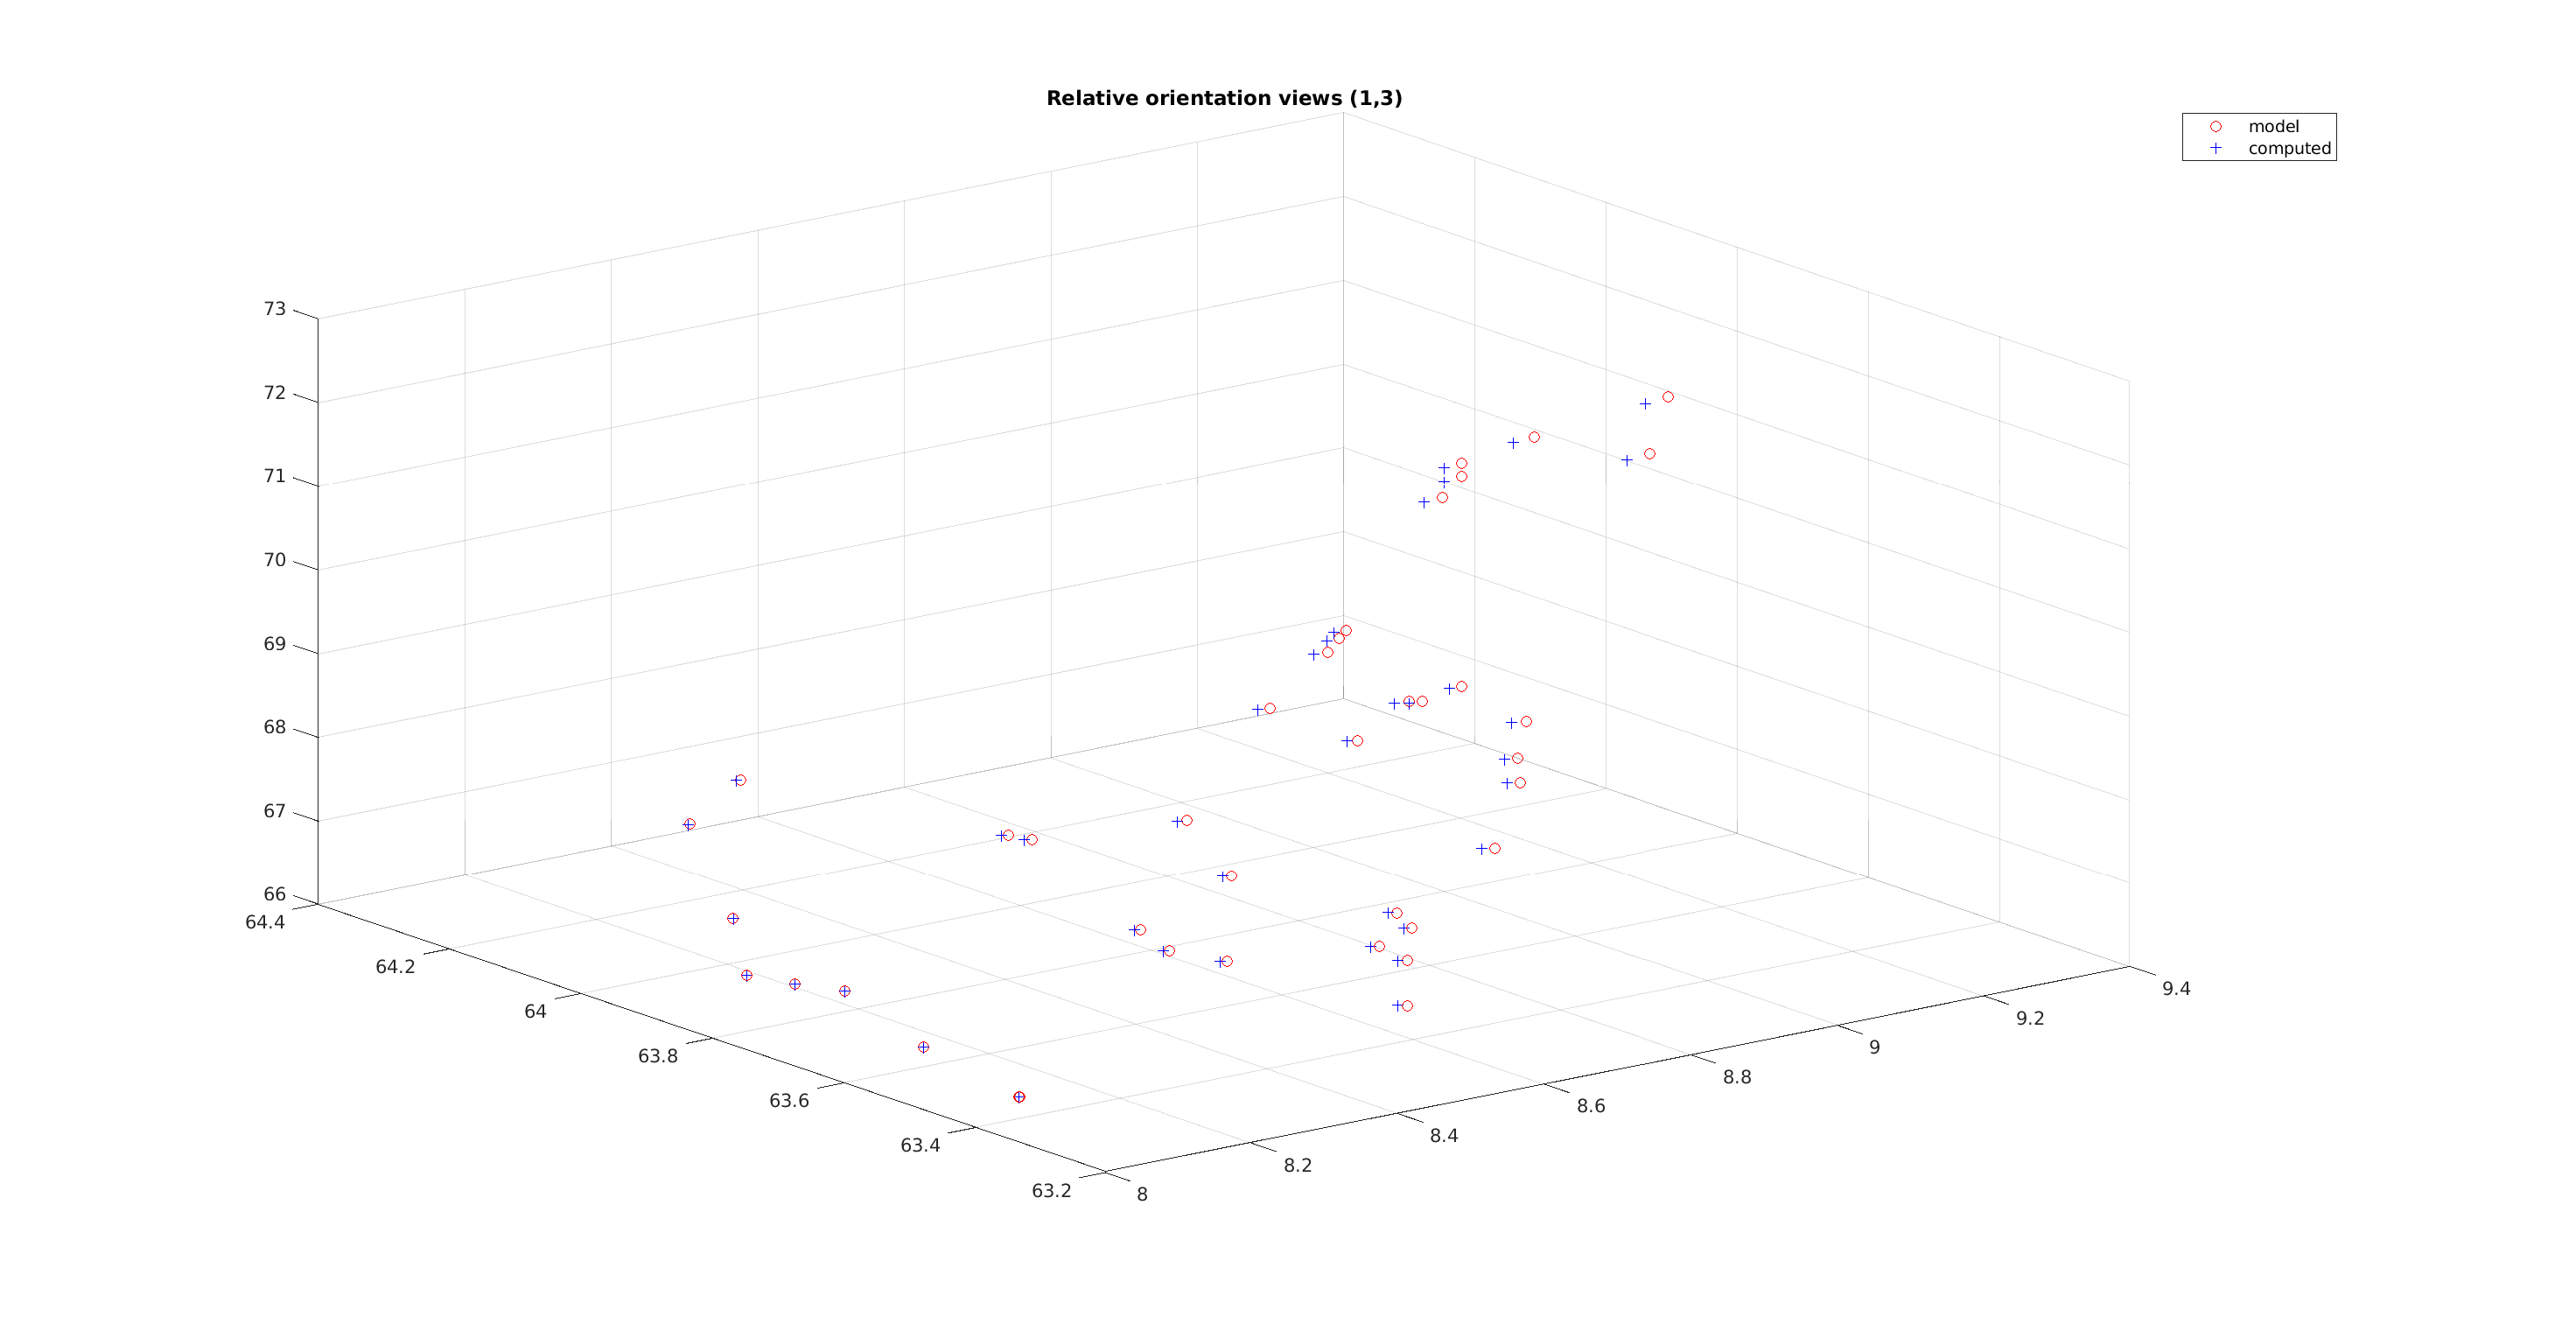
\includegraphics[scale=0.45]{images/relative_2.eps}
    \qquad 
    \qquad
    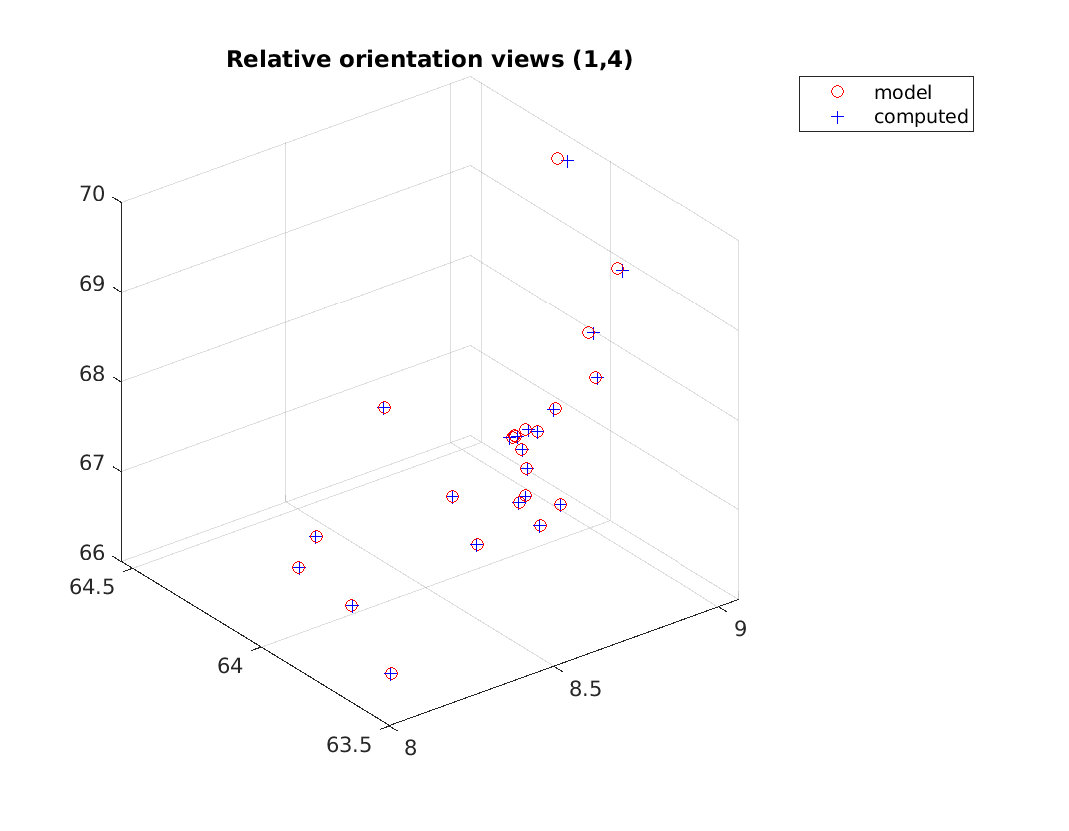
\includegraphics[scale=0.45]{images/relative_3.eps}
    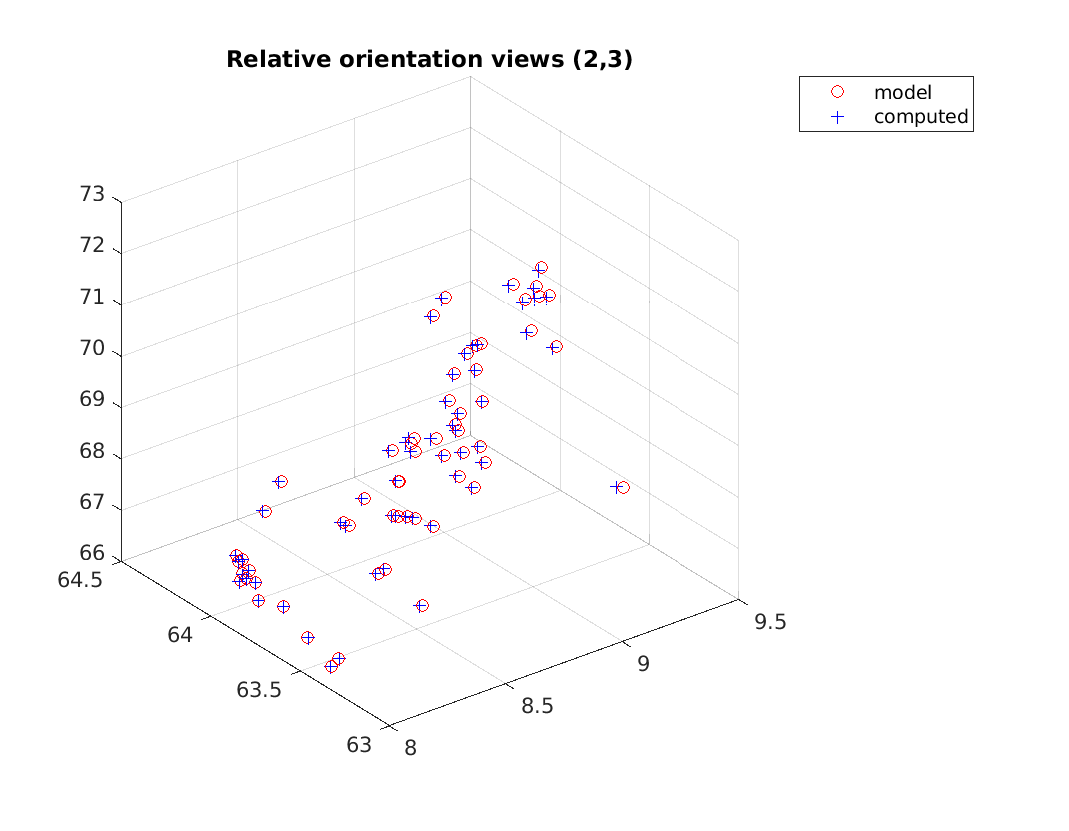
\includegraphics[scale=0.45]{images/relative_4.eps}
    \caption{Example of orientations with OPA of the 3D points of the model and the computed ones. The considered views are reported in the images.}
    \label{fig:relative}
\end{figure}

\begin{figure}[H]
    \centering
    \hspace*{-7cm}
    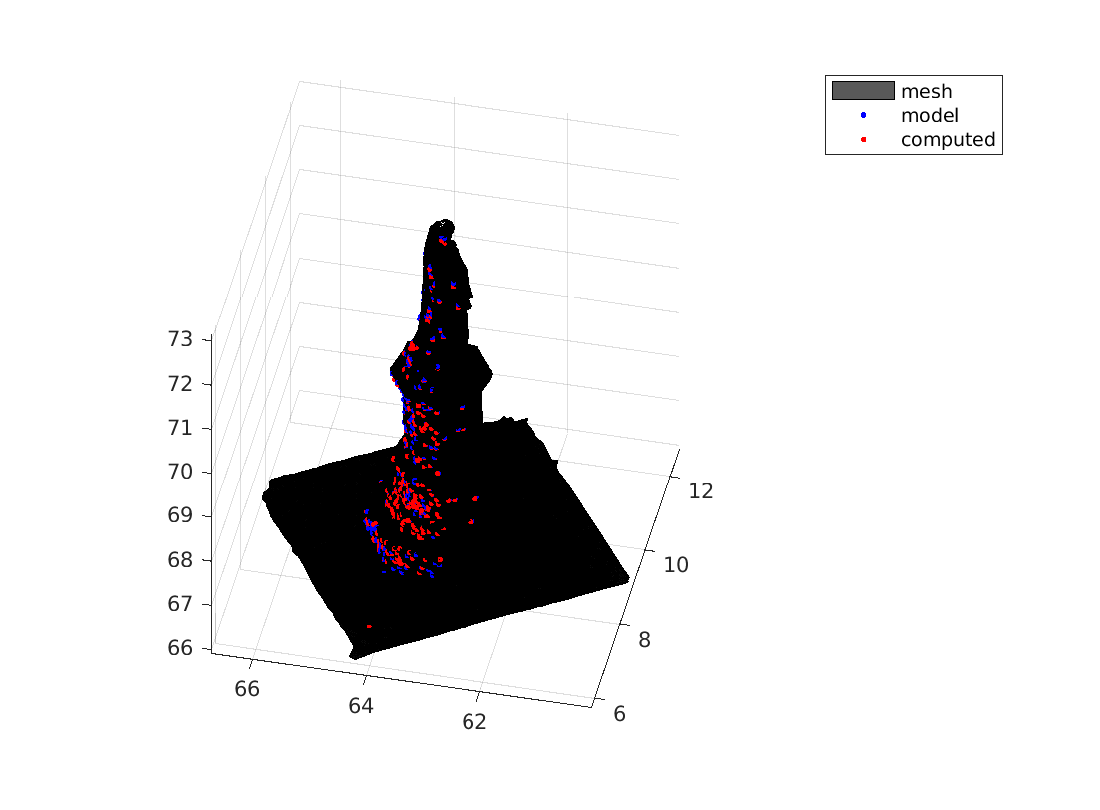
\includegraphics[scale=0.65]{images/statue.eps}
    \caption{Final result using 5 views}
    \label{fig:statue}
\end{figure}

\section{Final considerations}
This project proposed a minimal pipeline to try auto-calibration algorithms. Three algorithms are presented and the problems related to the correct estimation of the fundamental matrices and the initial estimation has been briefly discussed. It is clear that a good initial estimation is necessary and ad-hoc consideration for the optimizations and the number of fundamental matrices are required. Other more advanced methods can be considered like the one proposed in \cite{Gherardi10} to make the entire process more robust and reliable. 

\section{Appendix A: Sample execution of the pipelines}
\noindent The file \textit{pipeline\_dataset.m} will simply save the cell \textit{S.mat} with the previously explained fields.

\bigskip
\noindent The file \textit{pipeline\_autocalibration.m} starting from the dataset and the cell previously computed will display the previously discussed images and some logs to show all the steps. An example is reported:
\begin{verbatim}
    >> pipeline_autocal
    Pipeline for autocalibration starting from S data-structure
    Computing fundamental matrices
    Fundamental nonlin Smps error views (1, 2):	 0.14348 
    Fundamental nonlin Smps error views (1, 3):	 0.14054 
    Fundamental nonlin Smps error views (1, 4):	 0.1471 
    Fundamental nonlin Smps error views (1, 5):	 0.14393 
    Fundamental nonlin Smps error views (1, 6):	 0.14736 
    Fundamental nonlin Smps error views (1, 7):	 0.14304 
    Fundamental nonlin Smps error views (2, 1):	 0.14348 
    Fundamental nonlin Smps error views (2, 3):	 0.14193 
    Fundamental nonlin Smps error views (2, 4):	 0.14217 
    Fundamental nonlin Smps error views (2, 5):	 0.14069 
    Fundamental nonlin Smps error views (2, 6):	 0.14432 
    Fundamental nonlin Smps error views (2, 7):	 0.14286 
    Fundamental nonlin Smps error views (3, 1):	 0.14054 
    Fundamental nonlin Smps error views (3, 2):	 0.14193 
    Fundamental nonlin Smps error views (3, 4):	 0.13951 
    Fundamental nonlin Smps error views (3, 5):	 0.14084 
    Fundamental nonlin Smps error views (3, 6):	 0.1438 
    Fundamental nonlin Smps error views (3, 7):	 0.14463 
    Fundamental nonlin Smps error views (4, 1):	 0.1471 
    Fundamental nonlin Smps error views (4, 2):	 0.14217 
    Fundamental nonlin Smps error views (4, 3):	 0.13951 
    Fundamental nonlin Smps error views (4, 5):	 0.1451 
    Fundamental nonlin Smps error views (4, 6):	 0.14475 
    Fundamental nonlin Smps error views (4, 7):	 0.1425 
    Fundamental nonlin Smps error views (4, 8):	 0.14032 
    Fundamental nonlin Smps error views (4, 9):	 0.13927 
    Fundamental nonlin Smps error views (5, 1):	 0.14393 
    Fundamental nonlin Smps error views (5, 2):	 0.14069 
    Fundamental nonlin Smps error views (5, 3):	 0.14084 
    Fundamental nonlin Smps error views (5, 4):	 0.1451 
    Fundamental nonlin Smps error views (5, 6):	 0.14105 
    Fundamental nonlin Smps error views (5, 7):	 0.13864 
    Fundamental nonlin Smps error views (5, 8):	 0.14511 
    Fundamental nonlin Smps error views (5, 9):	 0.13984 
    Fundamental nonlin Smps error views (5, 10):	 0.14576 
    Fundamental nonlin Smps error views (6, 1):	 0.14736 
    Fundamental nonlin Smps error views (6, 2):	 0.14432 
    Fundamental nonlin Smps error views (6, 3):	 0.1438 
    Fundamental nonlin Smps error views (6, 4):	 0.14475 
    Fundamental nonlin Smps error views (6, 5):	 0.14105 
    Fundamental nonlin Smps error views (6, 7):	 0.14097 
    Fundamental nonlin Smps error views (6, 8):	 0.1413 
    Fundamental nonlin Smps error views (6, 9):	 0.1446 
    Fundamental nonlin Smps error views (6, 10):	 0.14202 
    Fundamental nonlin Smps error views (7, 1):	 0.14304 
    Fundamental nonlin Smps error views (7, 2):	 0.14286 
    Fundamental nonlin Smps error views (7, 3):	 0.14463 
    Fundamental nonlin Smps error views (7, 4):	 0.1425 
    Fundamental nonlin Smps error views (7, 5):	 0.13864 
    Fundamental nonlin Smps error views (7, 6):	 0.14097 
    Fundamental nonlin Smps error views (7, 8):	 0.14224 
    Fundamental nonlin Smps error views (7, 9):	 0.13886 
    Fundamental nonlin Smps error views (7, 10):	 0.14415 
    Fundamental nonlin Smps error views (8, 4):	 0.14032 
    Fundamental nonlin Smps error views (8, 5):	 0.14511 
    Fundamental nonlin Smps error views (8, 6):	 0.1413 
    Fundamental nonlin Smps error views (8, 7):	 0.14224 
    Fundamental nonlin Smps error views (8, 9):	 0.14576 
    Fundamental nonlin Smps error views (8, 10):	 0.14728 
    Fundamental nonlin Smps error views (9, 4):	 0.13927 
    Fundamental nonlin Smps error views (9, 5):	 0.13984 
    Fundamental nonlin Smps error views (9, 6):	 0.1446 
    Fundamental nonlin Smps error views (9, 7):	 0.13886 
    Fundamental nonlin Smps error views (9, 8):	 0.14576 
    Fundamental nonlin Smps error views (9, 10):	 0.14381 
    Fundamental nonlin Smps error views (10, 5):	 0.14576 
    Fundamental nonlin Smps error views (10, 6):	 0.14202 
    Fundamental nonlin Smps error views (10, 7):	 0.14415 
    Fundamental nonlin Smps error views (10, 8):	 0.14728 
    Fundamental nonlin Smps error views (10, 9):	 0.14381 
    Estimating intrinsic parameters
    Original
       1.0e+03 *
    
        5.7942         0    2.7923
             0    5.7942    1.8174
             0         0    0.0010
    
    Initial estimation
       1.0e+03 *
    
        5.9410         0    2.7360
             0    5.9410    1.8240
             0         0    0.0010
    
    Medonca cipolla: 
       1.0e+03 *
    
        5.9209    0.0017    2.7613
             0    5.8837    1.8216
             0         0    0.0010
    
    Autocalibration % error:	 2.1854 
    
    Kruppas method: 
       1.0e+03 *
    
        5.9410    0.0022    2.7361
             0    5.9409    1.8256
             0         0    0.0010
    
    Autocalibration % error:	 2.5332 
    
    Medonca cipolla (Toolbox): 
       1.0e+03 *
    
        5.8317         0    2.7673
             0    5.8317    1.8225
             0         0    0.0010
    
    Autocalibration % error:	 0.64652 
    
    Computing relative orientations of views
    Relative linear SO3 views (1, 2) error:	 0.0056306 
    Relative nonlin SO3 views (1, 2) error:	 0.0057026 
    Relative triang error views (1, 2):	 0.027706 
    Relative linear SO3 views (1, 3) error:	 0.012186 
    Relative nonlin SO3 views (1, 3) error:	 0.012521 
    Relative triang error views (1, 3):	 0.012344 
    Relative linear SO3 views (1, 4) error:	 0.018683 
    Relative nonlin SO3 views (1, 4) error:	 0.018827 
    Relative triang error views (1, 4):	 0.0047162 
    Relative linear SO3 views (1, 5) error:	 0.022338 
    Relative nonlin SO3 views (1, 5) error:	 0.022124 
    Relative triang error views (1, 5):	 0.0088446 
    Relative linear SO3 views (2, 3) error:	 0.0075514 
    Relative nonlin SO3 views (2, 3) error:	 0.0076158 
    Relative triang error views (2, 3):	 0.032475 
    Relative linear SO3 views (2, 4) error:	 0.014764 
    Relative nonlin SO3 views (2, 4) error:	 0.014717 
    Relative triang error views (2, 4):	 0.0073654 
    Relative linear SO3 views (2, 5) error:	 0.019423 
    Relative nonlin SO3 views (2, 5) error:	 0.019609 
    Relative triang error views (2, 5):	 0.0063714 
    Relative linear SO3 views (3, 4) error:	 0.0074843 
    Relative nonlin SO3 views (3, 4) error:	 0.0074571 
    Relative triang error views (3, 4):	 0.03073 
    Relative linear SO3 views (3, 5) error:	 0.013501 
    Relative nonlin SO3 views (3, 5) error:	 0.013511 
    Relative triang error views (3, 5):	 0.010332 
    Relative linear SO3 views (4, 5) error:	 0.0061366 
    Relative nonlin SO3 views (4, 5) error:	 0.0060958 
    Relative triang error views (4, 5):	 0.017958 
    Computing final points by view concatenation
    Relative triang error views (1, 2):		 0.027706 
    Relative triang error views (1, 3):		 0.012344 
    Relative triang error views (1, 4):		 0.0047162 
    Relative triang error views (1, 5):		 0.0088446 
    Relative triang error views (2, 3):		 0.032475 
    Relative triang error views (2, 4):		 0.0073654 
    Relative triang error views (2, 5):		 0.0063714 
    Relative triang error views (3, 4):		 0.03073 
    Relative triang error views (3, 5):		 0.010332 
    Relative triang error views (4, 5):		 0.017958 
    Pipeline completed
\end{verbatim}

\begin{thebibliography}{100}
    \addtolength{\leftmargin}{0.2in}
    \setlength{\itemindent}{-0.2in}

    \bibitem{Gherardi10} Riccardo Gherardi and Andrea Fusiello "Practical Autocalibration", ECCV10
    \bibitem{Medonca99} Medonca and Cipolla A Simple Technique for Self-Calibration
    \bibitem{Prapitasari14} A Study of Kruppa’s Equation for Camera Self-calibration
    \bibitem{Faugeras89} Huang T. and Faugeras O. Some properties of the E matrix in two-view motion estimation. 
    \bibitem{Dante} Dante Dataset https://www.3dflow.net/3df-zephyr-reconstruction-showcase/
    \bibitem{Hartley95} Hartley R. I. (1995). In defence of the 8-point algorithm.
    \bibitem{Fusiello} Andrea Fusiello Visione computazionale. Tecniche di ricostruzione tridimensionale
    \bibitem{Luong} Luong Q.-T.; Faugeras O. D. (1996). The fundamental matrix: Theory, algorithms, and stability analysis.
    \bibitem{Pollefeys} M. Pollefeys and L.V. Gool Stratified Self-Calibration with the Modulus Constraint
\end{thebibliography}

\end{document}